\chapter[Fundamentação]{Fundamentação}
\addcontentsline{toc}{chapter}{Fundamentação}

  \section{Metodologia de desenvolvimento}
  
  A metodologia de desenvolvimento adotada neste projeto é uma adaptação de metodologias gerais de desenvolvimento de
  produtos e serviços. Para a construção deste modelo de desenvolvimento foram selecionadas algumas técnicas de projeto
  de produtos e serviços expostos em algumas obras de Slack (\citeyear{slack99}), Krajewski (\citeyear{krajewski96}) e
  Ramaswamy (\citeyear{ramaswamy96}). Tais trabalhos descrevem formas de estabelecer etapas bem definidas para o desenvolvimento do projeto.
  
  Como estrutura básica do projeto será adotada a seguinte metodologia, dividida em seis etapas:
  
  \begin{figure}[h]
  \begin{center}

  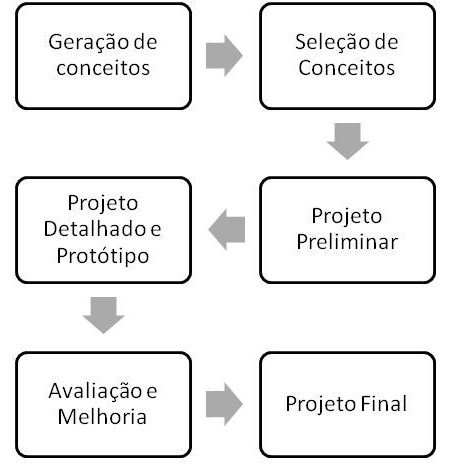
\includegraphics[scale=0.3]{editaveis/figuras/metodologia_de_desenvolvimento}
  \label{Metodologia de desenvolvimento}
  \caption{Metodologia de desenvolvimento}
  \end{center}
  \end{figure}
  \FloatBarrier
  
  A descrição de todas as etapas a cima é relatada a seguir.
  
  \begin{enumerate}
   \parindent=1.25cm
   
   \item Geração de Conceito\\
      
      \noindent
      Divide-se em três:
      
      \noindent
      \subitem \textbf{Geração de ideias}
      
      Foi proposto ao grupo o desenvolvimento de um projeto preliminar de uma planta de abastecimento de água potável a partir 
      da umidade do ar. O projeto a ser realizado deveria ser inovador, de utilidade para seus consumidores finais, viável e
      que utilizasse fontes alternativas de energia para a solução do problema a ser idealizado pelo grupo.
      
      O método utilizado nesta etapa do projeto consiste em produzir reuniões onde todo o grupo estará presente, tais componentes 
      devem fornecer ideias que possam ser debatidas e analisadas por todos, sem descriminação.
      
      \noindent
      \subitem \textbf{Análise de tecnologia}
      
      Nesta fase devem ser realizadas vigorosas pesquisas externas a fim de investigar a existência de tecnologias que realizam o
      trabalho proposto ou que realizam processos similares. 
	    
      A proposta desta etapa é investigar os prós e contras das várias tecnologias pesquisadas e a viabilidade da tecnologia 
      a ser adotada.
      
      \noindent
      \subitem \textbf{Especificação de localização}
      
      Análise de requisitos sobre localização e avaliação das características do problema, a fim de identificar os possíveis 
      consumidores e sua localidade. 
      
      Os potenciais consumidores deste projeto são as famílias nordestinas, que tem suas vidas diariamente sendo ameaçadas 
      devido à falta de reserva de água.
   
  \item Seleção de Conceitos
  
    Esta etapa é responsável por avaliar quais conceitos gerados na fase anterior são relevantes e pela construção do
    embasamento teórico sobre os elementos determinados na etapa anterior. 
  
  \item Projeto Preliminar
  
    Esta etapa busca especificar o serviço e o produto com todos os seus componentes e processos necessários ao funcionamento.
    
    Esta fase é uma das mais importantes de todo o projeto, pois são tomadas decisões que serão o suporte de todo o
    desenvolvimento deste. No projeto preliminar deste projeto foram estabelecidas as seguintes informações principais: 
    
    \begin{itemize}
     \item A região de implementação do projeto será no Município de Acari, situado mais especificamente na região do Seridó, 
	na Mesorregião Central Potiguar, no estado do Rio Grande do Norte, no Brasil.
     
     \item A tecnologia adotada será uma turbina eólica capaz de transformar a umidade do ar em água.
     
     \item Serão adotados critérios quanto a qualidade da água, eficiência da turbina e 
	monitoramento de todo o sistema de captação, armazenamento e distribuição.     
    \end{itemize}
    
  \item Projeto Detalhado e Protótipo
  
    O projeto detalhado se diferencia do projeto preliminar devido às alterações e correções implementadas.
    
    O protótipo do projeto será feito na plataforma de desenho Catia v5\_R19, este processo de construção deve ter como 
    base o projeto detalhado e as dimensões reais do produto, para ser feito em menor escala.

  \item Avaliação e Melhoria
  
    Antes do término do projeto e lançamento do serviço, algumas modificações devem ser feitas em busca de melhorias. 
    Dentre as técnicas utilizadas neste processo, serão recomendadas o Desdobramento da Função Qualidade
    (ou QFD, Quality Function Deployment) e da Análise de Valor.
    
    O Desdobramento da Função Qualidade (QFD) tem como foco principal às necessidades dos clientes, oferecendo as
    alternativas capazes de satisfazê-los. Ou seja, dentro da matriz QFD os requisitos do consumidor (o quê) relacionam-se
    com as características do serviço (como), para que possamos prover mudanças que aumentem a satisfação do cliente.
    
    A Análise de Valor tem como objetivo aumentar o valor relativo de cada componente do serviço prestado, o que pode 
    ser feito através da redução de custos ou através do aumento do nível do serviço. Deve-se, em uma primeira etapa,
    distinguir as funções básicas das secundárias, para em seguida identificar tudo o que possa oferecer diminuição de custos,
    principalmente em funções secundárias; e aumento do valor, em funções básicas.
    
  \item Projeto Final
  
    O projeto final deve conter as alterações propostas por meio das técnicas de avaliação e melhoria, em modelo semelhante
    ao do projeto preliminar, porém de forma extremamente mais completa.
    
  \end{enumerate}

  
  \section{Referencial Teórico}
  
    Essa seção aborda alguns conceitos chave referentes ao trabalho.
    
    \subsection{Sistema de captação da umidade do ar}
    
      \documentclass[12pt,openright,oneside,a4paper,brazil]{abntex2}
\usepackage[utf8]{inputenc}
\counterwithout{section}{section}
\counterwithout{figure}{chapter}
\counterwithout{table}{chapter}
\setlength{\parindent}{1.3cm}
\usepackage{indentfirst}
\setlength{\parskip}{0.2cm}
\usepackage[bottom=2cm,top=3cm,left=3cm,right=2cm]{geometry}
\usepackage{graphicx}
\graphicspath{{figuras/}}
\usepackage{placeins}
\usepackage{cite}
\usepackage{url}
\usepackage{breakurl}
\include{bibliografia}

\makeatletter
\setlength{\@fptop}{0pt}
\makeatother

\begin{document}

\textual
\begin{center}
 {\large Captação de água e materiais estruturais}\\[0.2cm]
 \end{center}
 
Dentre as inspirações de tecnologia a serem aplicadas no projeto, as que se destacaram foram a Eolewater, Maxwater, Skywater e Warkawater. As três primeiras se baseiam no cooling compression, porém com custos diferentes. A Quarta tem custo  extremamente baixo se comparado com as outras Três tecnologias, por causa da simplicidade dos materiais que a constituem.Contudo, produz valores significantemente menores de água, além de não gerar energia para os processos de controle da qualidade da água. Por não gerar energia, também descartamos o Skywater.

As duas primeiras se baseiam em turbinas eólicas autossuficientes que retiram a umidade do ar, condensam, purificam e distribuem. Devido a geometria dos rotores do Max water que não é tão eficiente como os rotores tradicionais, de turbinas eólicas comuns, foi escolhido como base O sistema da Eolewater, que está descrito na figura 2.

\begin{figure}[!ht]
\centering
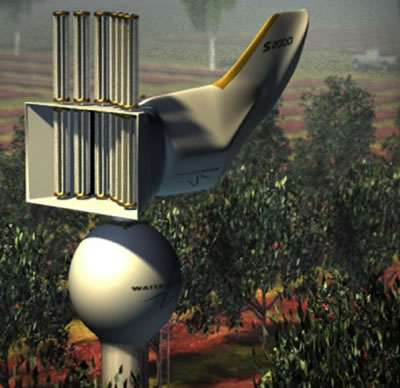
\includegraphics[scale=0.6]{max_water}
\caption[Caption title in LOF]{Max Water. Note como seus rotores são paralelos e verticais, tal configuração é ineficiente do ponto de vista aerodinâmico por gerar turbulência sobre os rotores vizinhos e gerar torques contrários com uma mesma direção de fluxo de ar.\footnotemark}

\label{Max_Water}
\end{figure}
\footnotetext{Disponível em: http://peswiki.com/index.php/Image:Max-water.jpg}

\begin{figure}[!htbp]
\centering
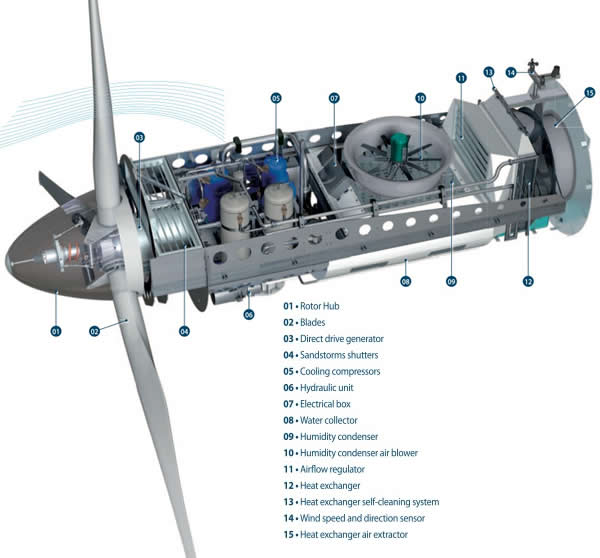
\includegraphics[scale=0.6]{Componentes}
\caption[Caption title in LOF]{Componentes de uma turbina Eolewater.\footnotemark}
\FloatBarrier
\label{Max_Water}
\end{figure}

\footnotetext{Fonte: RENEWABLE ENERGY DEVELOPMENT, 2012 }

As componentes de uma turbina eólica pouco mudam para essa acima,pois a Eolewater além de gerar energia para seu próprio funcionamento gera água, enquanto que a turbina eólica gera apenas energia.Na maioria das tecnologias de sucesso que pesquisamos, A Obtenção de água é feita pela condensação  a frio (cooling condensation), que é feita com o contato de ar com uma superfície fria. Para gerar essa superfície fria, um compressor comprime um fluido refrigerante, elevando sua temperatura. Esse fluido em alta temperatura passa por um trocador de calor e depois é expandido, o que causa uma queda ainda maior na temperatura do fluido. O fluido sob baixa temperatura circula por um condensador, por onde passa o ar atmosférico coletado. Esse condensador faz com que a temperatura do ar caia até o ponto de orvalho, temperatura na qual a água presente no ar se condensa em pequenas gotículas devido a saturação da quantidade de água no ar. A água proveniente da condensação é coletada e passa por tratamentos em UV e carvão ativado para que seja descontaminada e esteja pronta para consumo.



No Momento, o levantamento de materiais será apenas estrutural e se baseará em uma turbina eólica.

\begin{figure}[!htbp]
\centering
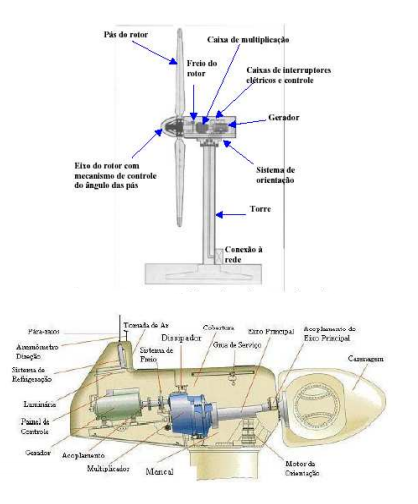
\includegraphics[scale=0.80]{turbina}
\caption[Caption title in LOF]{Seção de uma turbina eólica típica conectada à rede.\footnotemark}
\FloatBarrier
\label{Max_Water}
\end{figure}
\footnotetext{Fonte: USP, 2005 }

Dentro da turbina eólica temos os seguintes subconjuntos: torre, rotor, nacele, caixa de multiplicação (transmissão), gerador, mecanismos de controle, anemômetro, pás de rotor, biruta (sensor de direção). A torre é o elemento que sustenta o rotor e a nacele na altura adequada para o funcionamento da turbina eólica. Esse item é de elevada contribuição no custo inicial do sistema. O rotor é a componente onde as pás são conectadas e que realiza a transformação de energia cinética dos ventos em energia mecânica de rotação (ROSSI; OLIVEIRA; ALÉ, 2015).

	Nacele é um compartimento localizado no alto da torre que abrigam mecanismos do gerador (freios, caixa multiplicadora, embreagens, sistemas hidráulico, etc). Usaremos a Nacele para também abrigar os mecanismos de obtenção de água. 
	
	Caixa multiplicadora (transmissão) é o mecanismo que transmite a energia mecânica do eixo do rotar ao eixo do gerador. Gerador é o converterá energia mecânica do eixo em energia elétrica. Mecanismos de controle são os que supervisionam a velocidade média nominal que ocorre com maior frequência durante um determinado período. Anemômetro tem a função de medir a intensidade e a velocidade dos ventos. Pás do rotor captam o vento e converte sua potência ao centro do rotor. Biruta é um conjunto de sensores que captam a direção do vento (ROSSI; OLIVEIRA; ALÉ, 2015).
	
	Uma das componentes que se tem muito estudo é a pá rotativa. Ela pode ser feita com os seguintes materiais: madeira, aço, alumínio, fibra de vidro com resina poliéster, fibra de vidro com fibra de carbono, madeira com epóxi, fibra de carbono. A escolha do material vai depender da escolha do perfil aerodinâmico, que será estudado posteriormente. (PORTAL ENERGIA, 2015).
\begin{figure}[!htbp]
\centering
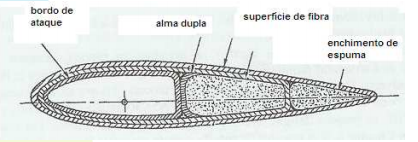
\includegraphics[scale=0.80]{pa}
\caption[Caption title in LOF]{Seção transversal de uma pá feita de fibra de vidro\footnotemark}
\FloatBarrier
\label{Max_Water}
\end{figure}
\footnotetext{Fonte: USP, 2005 }

Como pode ser visto as fibras são colocadas estruturalmente nas principais direções de propagação das tensões, quando em operação. A fibra de carbono e ou Kevlar são atualmente os compostos mais avançados que podem ser utilizados me áreas críticas (longarina da pá), mas tal material trem preços muito elevados (BARROS; VARELLA, 2015).  

Em relação ao suporte estrutural, ou torre, nas turbinas eólicas elas podem ser do tipo treliçadas, tubular e estaiada, no entanto, para a Eolewater as estruturas mais comuns são as duas últimas. As tores são constituídas de concreto e aço, tendo o peso em torno de 40 toneladas e 50 metros de comprimento (USP, 2005).

\begin{figure}[!htbp]
\centering
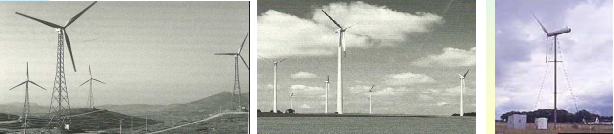
\includegraphics[scale=0.80]{torre}
\caption[Caption title in LOF]{Tipos de torre. Da esquerda para a direita: Treliçada, Tubular e Estaiada \footnotemark}
\FloatBarrier
\label{torre}
\end{figure}
\footnotetext{Fonte: USP, 2005 }

O modelo do dispositivo da Eolewater de gerar água por meio da energia eólica possui uma turbina WMS1000, de potência de30kW. O tempo de vida proposto para esse mecanismo é de 20 anos, dependendo das condições em que o motor é submetido ele pode gerar até 1200 litros de água por dia (mais informações na tabela abaixo). Como o dispositivo não necessita de quaisquer outros recursos para operar há um impacto mínimo sobre o meio em que é colocado (RENEWABLE ENERGY DEVELOPMENT, 2012).

\begin{figure}[!htbp]
\centering
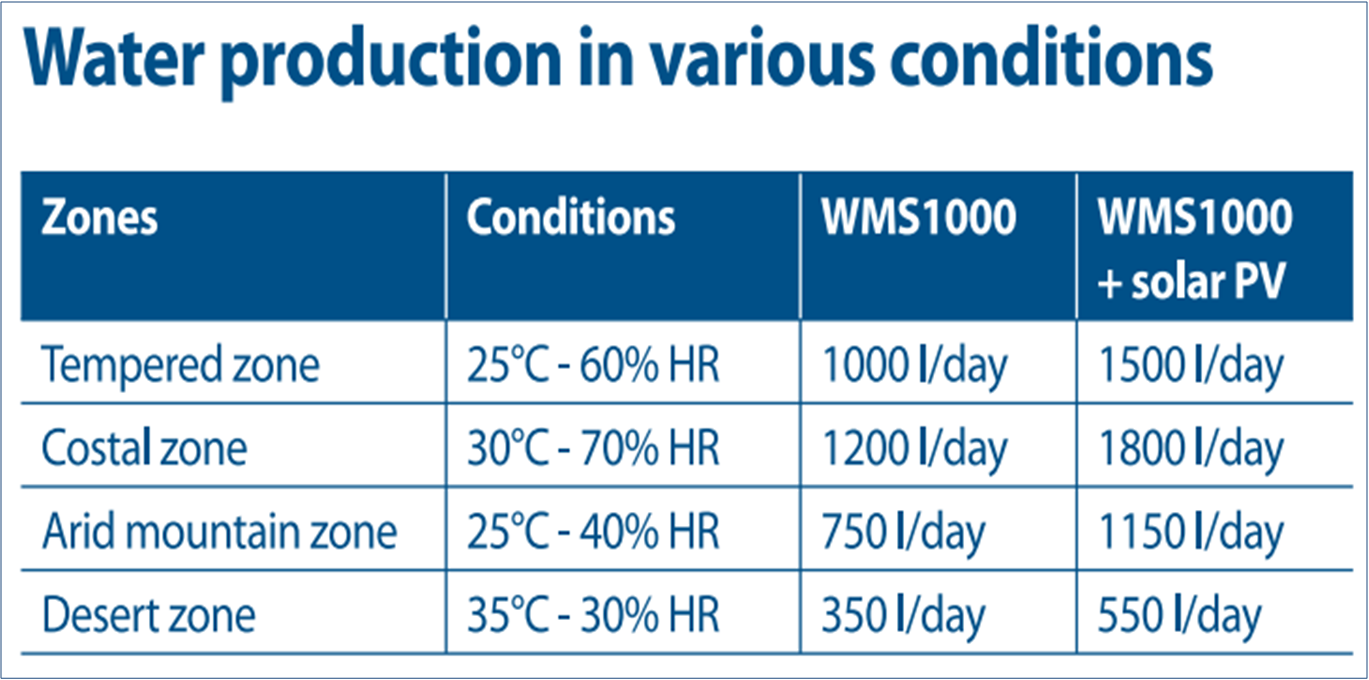
\includegraphics[scale=0.3]{condicoes}
\caption[Caption title in LOF]{Tabela de condições de umidade e temperatura para o rendimento de água \footnotemark}
\FloatBarrier
\label{condicoes}
\end{figure}
\footnotetext{Fonte: RENEWABLE ENERGY DEVELOPMENT, 2012}

Essa tecnologia possui um controle de pitch centrífuga para regular a velocidade do motor, tem um sistema de travagem rotor mecânica e elétrica, o qual evita danos nas lâminas giratórias (pás), ainda, contém um mastro de inclinação que integra a ação dos cilindros telescópicos com capacidade de empuxo de 115 toneladas. Deve-se destacar que os componentes que entram em contato com a água são feitos de uma liga de aço inoxidável especial que operará sem risco de corrosão (EOLE ÁGUA SAS, 2015).

	Uma tecnologia como essa segundo o site da Indústria Eólica uma turbina de vento abaixo de 100 kW vai custa por volta de US \$ 3.000 a US \$ 5.000  por quilowatt de capacidade. Portanto, levando em conta as especificações técnicas do Turbine WMS1000 abaixo a tecnologia é eficiente, mas cara (RENEWABLE ENERGY DEVELOPMENT, 2012).
	
\begin{figure}[!htbp]
\centering
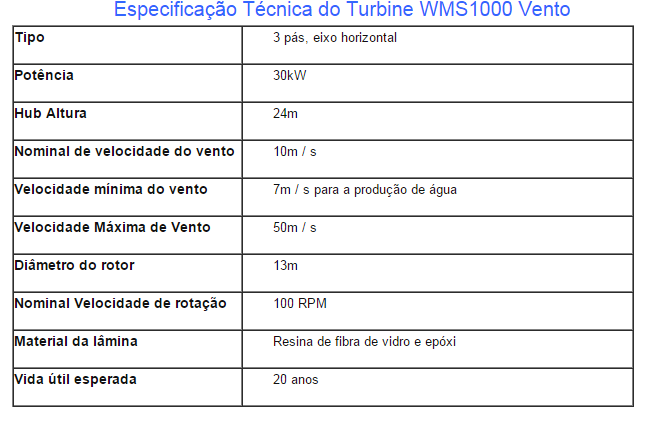
\includegraphics[scale=0.8]{especificacao}
\caption[Caption title in LOF]{Especificação Técnica do Turbine WMS1000 Vento \footnotemark}
\FloatBarrier
\label{Especificacoes}
\end{figure}
\footnotetext{Fonte: RENEWABLE ENERGY DEVELOPMENT, 2012}
 
A outra tecnologia, Warawater, por sua vez é uma tecnologia muito barata se comparada com a mencionada anterior. Essa custa cerca de US\$ 500 e pode ser construída em menos de uma semana com uma equipe de quatro pessoas e materiais existente localmente (DUARTE, 2015).

	Os materiais necessários para a sua construção de sua estrutura são: recipiente de coleta, bambu e um revestimento interno de plástico reciclado (rede). Sua torre possui em média 10 metros de altura, com 60 Kg e pode suprir até 100 litros de água por dia (TIMES, 2014).
\begin{figure}[!htbp]
\centering
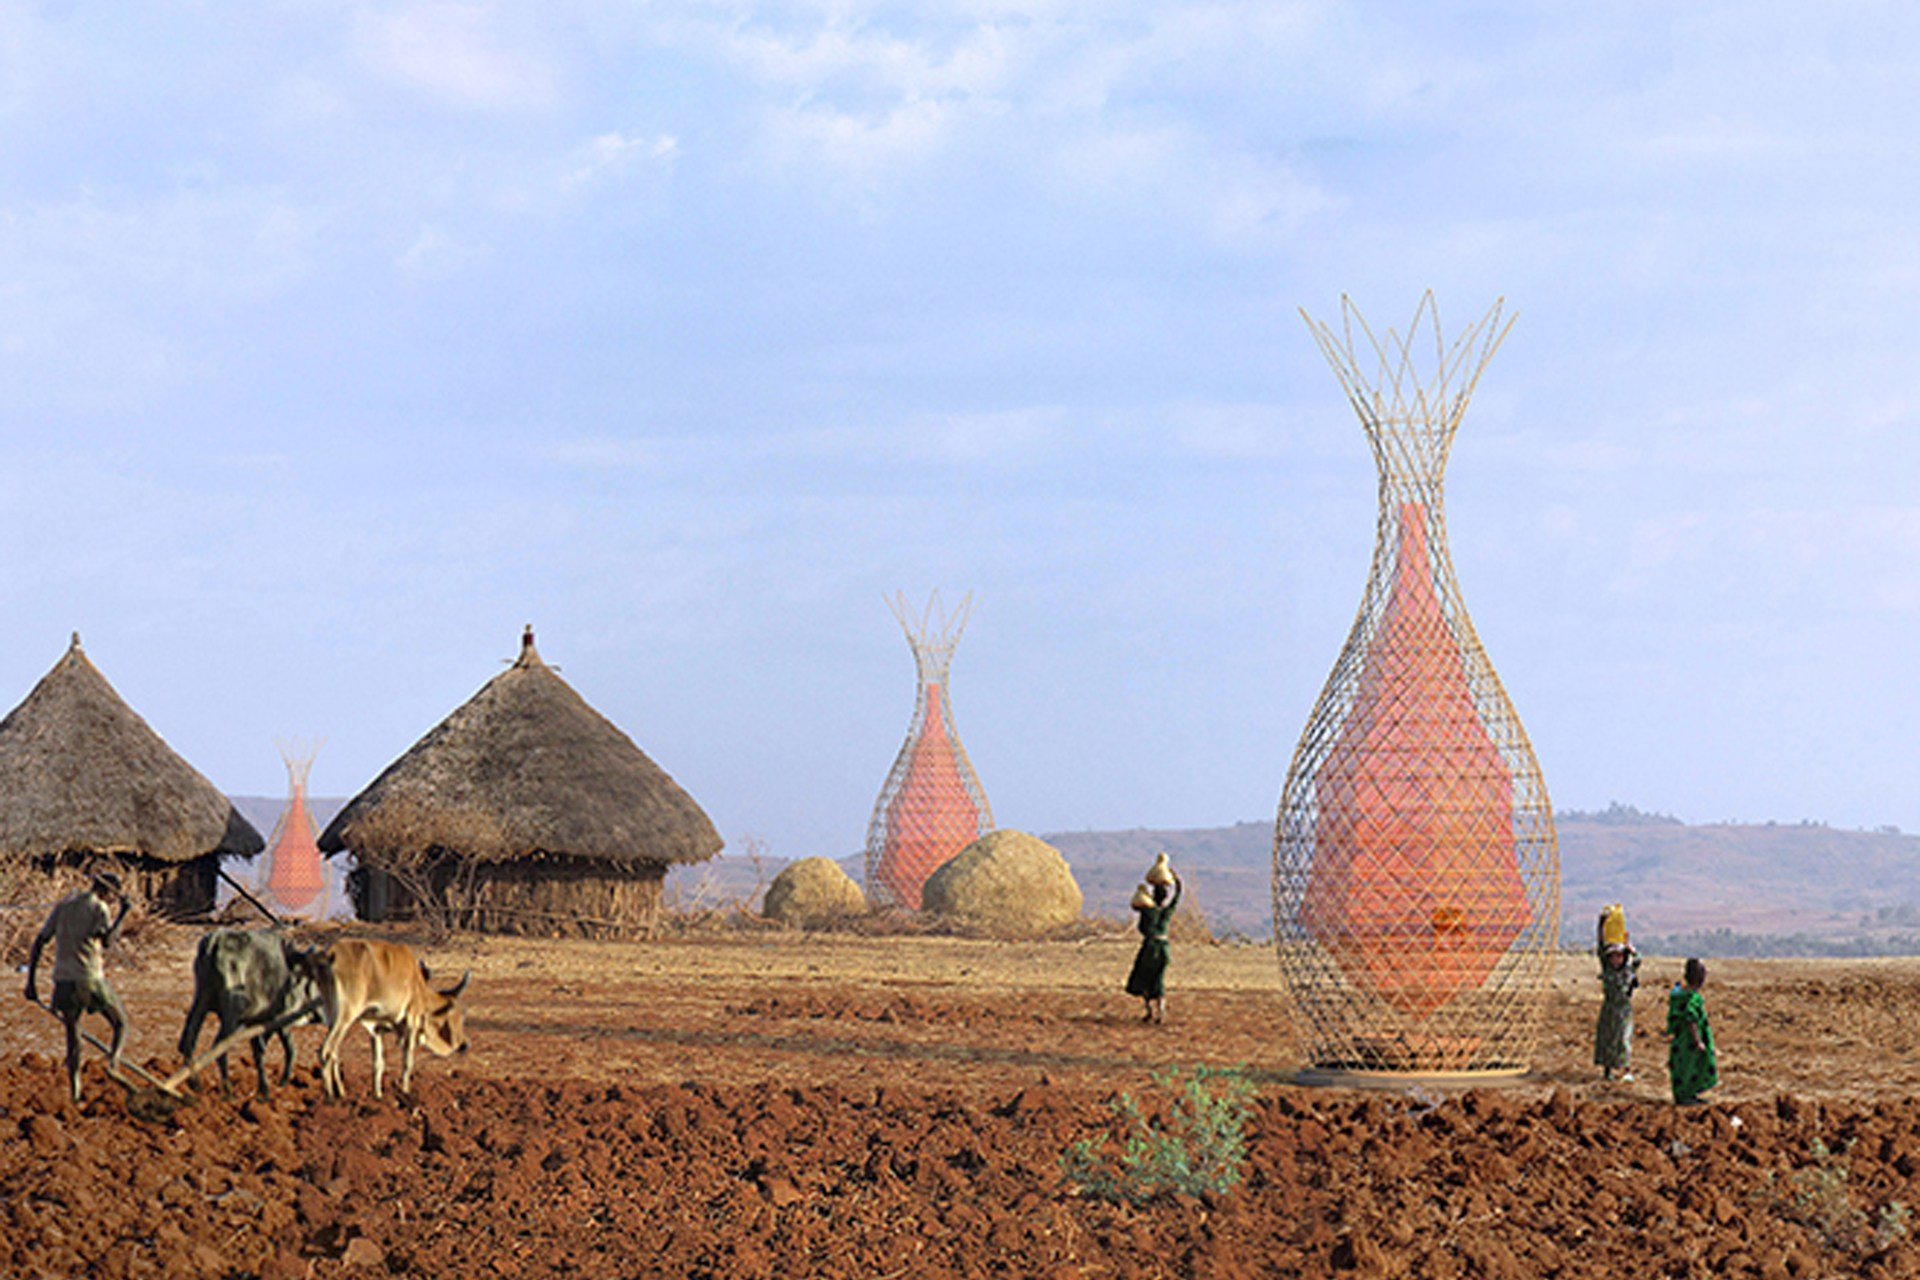
\includegraphics[scale=0.3]{warkawater}
\caption[Caption title in LOF]{Utilização da tecnologia warkawater por uma população carente  \footnotemark}
\FloatBarrier
\label{Especificacoes}
\end{figure}
\footnotetext{Fonte: DUARTE, 2015}

\bibliographystyle{abnt-alf}
\bibliography{bibliografia}

\end{document}
    
    \subsection{Matriz energética}
    
      Na contemporaneidade, quando se fala de geração de energia, em qualquer local do mundo a primeira questão a ser levantada
é a de maior distribuição possível juntamente com a maior viabilidade econômica envolvida. Estes foram dois parâmetros 
primordiais para se escolher a energia renovável para ser implantada dentro do projeto.

A Matriz Energética do Projeto foi divida em três áreas apresentadas a seguir.

  \subsubsection{Fontes Energéticas Referenciais}
    
    No decorrer do período de elaboração do escopo do projeto, várias possíveis soluções foram levantadas e, em seguida, 
    discutidas com o intuito de se chegar em um sistema que atendesse da melhor formar os requisitos iniciais do projeto.
    Dentre todas as opções disponíveis, foram pré-selecionadas três que, em princípio, se destacaram. São elas:
    
    \begin{itemize}
      \item \textbf{Eole Water}: uma turbina eólica autossuficiente que capta a água a partir de um sistema de refrigeração
	que faz com q a água no ar se condense ao entrar em contato com suas pás.
     
      \item \textbf{Maxwater}: um moinho de vento vertical, com um sistema muito semelhante ao primeiro, mas que possui custo,
	produção diferenciados.
      
      \item \textbf{Warkawater}:torre feita de bambu e que é forrada por dentro com uma malha plástica, que retém gotículas
	de orvalho. Esse sistema é passivo e não necessita de energia para produção de água já que funciona de forma passiva.
    \end{itemize}
  
    Dois requisitos muitos importantes para a escolha do sistema foram a necessidade do uso de uma fonte energética renovável
    e de que a água fosse analisada em tempo real. Observando o segundo requisito se percebe que existe a necessidade da
    implementação de sensores e de um sistema que envie todos os dados recolhidos por tais sensores. Nesse contexto pensou-se 
    primeiramente no uso de painéis solares fotovoltáicos, em um segundo momento, levando em consideração a região propícia à 
    implementação de um parque eólico e escolha do sistema Eolewater, decidiu-se por utilizar o excedente de energia gerado 
    pela turbina eólica para suprir as necessidades dos sistemas embarcados.
  
    A premissa do uso do potencial dos ventos para geração de trabalho data de milhares de anos atrás, onde essas tecnologias
    eram usadas principalmente para o bombeamento de água e para moagem de grãos. As primeiras tentativas do uso da energia
    eólica para geração de eletricidade foram no século XIX, ma só na década de 1970 é que essa tecnologia foi aplicada em
    escala comercial.
    
    A avaliação do potencial eólico de uma região requer trabalhos sistemáticos de coleta e análise de dados sobre a velocidade
    e o regime de ventos. Geralmente, uma avaliação rigorosa requer levantamentos específicos, mas dados coletados em 
    aeroportos, estações meteorológicas e outras aplicações similares podem fornecer uma primeira estimativa do potencial
    bruto ou teórico de aproveitamento da energia eólica.
    
    Embora ainda haja divergências entre especialistas e instituições na estimativa do potencial eólico brasileiro, 
    vários estudos indicam valores extremamente consideráveis. Até poucos anos, as estimativas eram da ordem de 20.000 MW.
    Hoje a maioria dos estudos indica valores maiores que 60.000 MW.
    
    As primeiras turbinas eólicas de uso comercial tinham a capacidade de produção elétrica entre 10kW e 50kW, já
    as máquinas de grande porte atuais tem uma potência superior a 1Mw. 
    
  \subsubsection{Técnicas e métodos de conversão e armazenamento}
    
    Um dos desafios do projeto foi estabelecer a demanda de água para a região selecionada e a partir disso dimensionar a
    estrutura física necessária de acordo com os requisitos. Dentre os modelos analisados pela equipe, a turbina de vento 
    mais favorável foi a Eolewater, modelo WMS100 Wind Turbine da empresa EoleWater, uma turbina de eixo horizontal que
    apresenta resultados satisfatórios à proposta e servirá de base de estudo para a implementação do projeto na área 
    energética.
    
    Apesar dos avanços nessa área, a energia eólica não possui uma capacidade de produção muito grande, por isso deve-se
    focar no requisito eficiência de conversão. Algumas formas de aperfeiçoar a produção estão relacionadas à dimensão do 
    gerador, aerodinâmica, materiais utilizados, projeção da estrutura e logística.
    
    Partindo dessa necessidade, o gerador exerce função primordial no funcionamento da turbina, pois é ele quem converte a
    energia mecânica em energia elétrica que alimenta todo o sistema. Dessa forma, temos o seguinte esquema de funcionamento:
    Os ventos fazem com que as pás do rotor girem, consequentemente girando o rotor. Este, por sua vez, converte a energia 
    cinética dos ventos em energia mecânica de rotação. Esse conjunto conectado a um eixo transmite essa rotação para o
    gerador. O gerador finalmente converte a energia mecânica em energia elétrica que alimenta todos os outros componentes
    eletrônicos (controle) e mecânicos da turbina.
    
    A produção de energia elétrica estimada da turbina é de aproximadamente 30kW (a produção real depende do diâmetro do rotor,
    rendimento do sistema, velocidade dos ventos, condições climáticas da região). Essa energia produzida alimentará os
    componentes da turbina e a energia remanescente será utilizada pela estação de controle e armazenada em baterias para
    que seja utilizada em situações emergenciais.
    
    Dessa forma, temos a seguinte distribuição energética:
    
    \begin{figure}[!ht]
    \centering
    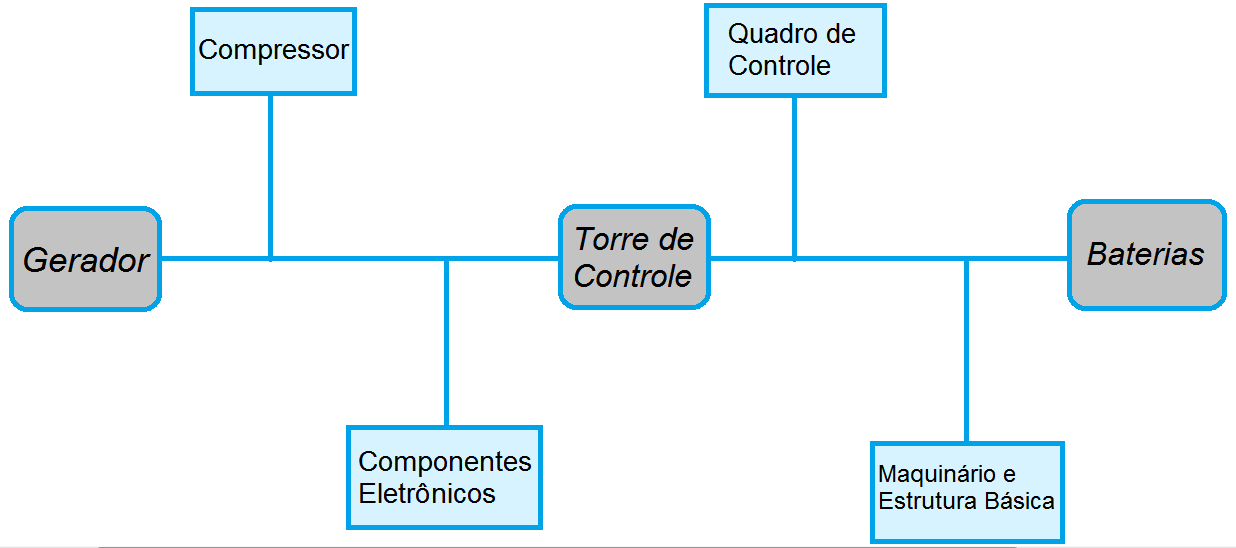
\includegraphics[scale=0.45]{editaveis/figuras/distribuicao_energetica}
    \caption{Distribuição energética}
    \label{distribuicao_energetica}
    \end{figure}
    
    \begin{enumerate}
     \item Geração de eletricidade (aproximadamente 30kW);
     \item Alimentação do compressor e componentes eletrônicos da turbina;
     \item Direcionamento a torre de controle;
     \item Distribuição no quadro de controle;
     \item Alimentação elétrica do maquinário e estrutura básica;
     \item Direcionamento de energia remanescente para as baterias emergenciais.
    \end{enumerate}
    
  \subsubsection{Eficiência Energética}
  
    A turbina eólica, ou aerogerador, é uma máquina capaz de absorver a potência cinética do vento por meio de um rotor
    aerodinâmico, convertendo este movimento em potência mecânica de eixo (torque vs rotação),  que é transformada em
    potência elétrica (tensão \textit{vs} corrente) por intermédio de um gerador elétrico.
    
    A parte estrutural de geração de energia de uma turbina é constituída por um rotor e pela torre que a sustenta,
    pela transmissão/multiplicação e pelo conversor. Ela somente consegue extrair energia através da energia cinética do 
    ar que passa pelo interior da área interceptada pelas pás rotativas.  
    
    Energia eólica provém da radiação solar. Se considerarmos que, aproximadamente, 2\% da energia solar que a Terra absorve,
    é convertida em energia cinética dos ventos, teremos uma estimativa da energia total disponível dos ventos ao redor
    do planeta.
    
    Os ventos (massas de ar em movimento),são influenciados por diferentes aspectos dentre os quais se destacam a rugosidade
    do solo, os obstáculos e o relevo da região, e possuem energia cinética que pode ser aproveitada com o uso de aerogeradores.
    
    Dessa forma, a energia cinética $E_C$, contida em uma amostra de volume de ar, $A$ x $\delta x$, com densidade do ar $\rho$, 
    movendo-se com uma velocidade, $v$,  onde $A$ é uma unidade de área perpendicular à direção dos ventos e $\delta x$ é paralelo 
    à direção dos  ventos, é dada por:
    
    $$ E_C = \frac{Mv^2}{2} = \frac{\rho A {\delta x} v^2}{2} $$
    
    A primeira vista, imagina-se que a máxima energia retirada dos ventos por uma turbina eólica é a energia cinética dos
    ventos que atravessam um círculo formado pela área das pás. Contudo, o próprio vento possui energia cinética na esteira
    do rotor, fazendo com que nem toda energia seja retirada. Segundo uma teoria criada por Betz* (para um modelo ideal), 
    a eficiência aerodinâmica do rotos estaria limitada a 59,3\% da energia presente nos ventos.
    
    O rotor é o primeiro estágio de conversão da energia do vento em eletricidade. Os estágios seguintes são a transmissão
    e o próprio gerador, que adéqua às velocidades de rotação e converte a energia mecânica em energia elétrica, 
    respectivamente.
    
    Em média, a eficiência de conversão dos modernos aerogeradores está dividida como ilustra a Figura ~\ref{eficiencia_conversao_aerogeradores}.
    
    \begin{figure}[!ht]
    \centering
    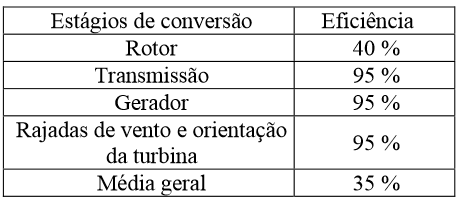
\includegraphics[scale=0.7]{editaveis/figuras/eficiencia_conversao_aerogeradores}
    \caption{Eficiência de conversão dos aerogeradores modernos}
    \label{eficiencia_conversao_aerogeradores}
    \end{figure}
    
    Na contemporaneidade, os parâmetros de rotores utilizados nos aerogeradores modernos são de duas ou três pás.
    Isso graças à relação de potência extraída por área de varredura do rotor (muito superior ao rotor multipás) para 
    velocidades mais elevadas. Tais características são aceitáveis em sistemas de geração de eletricidade, porém se tornam
    inviáveis em sistemas que requeiram altos momentos de força e/ou carga variável.
    
    Rotores modernos, com mais de três pás, são usados somente quando há necessidade de um grande torque de partida, ou seja, 
    basicamente, bombeamento mecânico de água. Aerodinamicamente, no entanto, grande número de pás e alto torque de partida,
    diminuem a eficiência do sistema. 

    Sendo assim, o desenvolvimento de pás para aerogeradores deve ser resultante da integração entre estes fatores.
    Com o estágio atual da tecnologia, a dificuldade de fabricação não reside na aerodinâmica, mas sim na construção
    e resistência dos materiais que compõem as pás, que devem responder a diferentes exigências da máquina eólica,
    além de ser necessário que sejam resistentes, rígidos, leves e de baixo custo.
    
    As perdas de transmissão relacionam-se diretamente ao atrito que existe entre as engrenagens.
    Em velocidades de giro fixas, as perdas variam pouco, podendo-se assumir que são uma porcentagem fixa
    da potência nominal. Esta porcentagem real depende da qualidade da transmissão, mas um valor razoável
    pode ser em torno de 2\% da potência em cada etapa de engrenamento. Como a transmissão consome certa quantidade de
    energia, as perdas podem ser consideráveis em baixas potências, já que o rendimento nestes casos é menor.
    
    Para que a geração de eletricidade a partir do movimento do ar seja plausível, técnica e economicamente, alguns fatores
    ganham relevância. A velocidade dos ventos é o fator mais crítico na determinação da energia que será obtida de um
    aerogerador, e também seu custo. Outros fatores seriam:
    \begin{itemize}
     \item \textbf{Topografia}: o ar é mais frio durante a noite e tende a ocupar regiões próximas ao solo, além de produzir
	pouca quantidade de vento. Por isso devem ser escolhidas áreas mais elevadas. Para a escolha dessas áreas devem ser
	observadas também: facilidade de locomoção até a instalação, proximidade ao ponto de consumo, espaço necessário
	para manutenções e evitar áreas muito frias, a fim de não danificar o aerogerador.
	
     \item \textbf{Barreiras Naturais}: prédios, árvores, plantações e construções elevadas que podem diminuir
	a velocidade do vento e turbulência, danificando o equipamento.
      
     \item \textbf{Superfície}: quanto mais acidentado o terreno (maior rugosidade), com plantações, construções, árvores, entre outros,
	mais alta a torre deve ser.
      
     \textit{Obs.:} Quando não especificada a altura na qual ocorreu a medição da velocidade dos ventos,
	consideramos a altura padrão internacional de 10 metros acima do solo, ou a altura em que cada gerador está operando. 
     
    \end{itemize}
    
    \subsection{Sistema de monitoramento e controle da qualidade da água}
      
      \subsubsection{Parâmetros de qualidade da água}
          
      \subsubsection{Projeto eletrônico e de controle da planta}
            
      \subsubsection{Interface do sistema de monitoramento da qualidade da água}
      
      
  \section{Requisitos do sistema}
  
      O projeto possui 4 frentes de requisitos. São elas:
      
      \begin{itemize}
	\item Requisitos do projeto estrutural mecânico do sistema de captação da água e do transporte para a central de armazenamento;\\
	 
	 \textbf{Requisitos funcionais}
	  \begin{itemize}
	   \item 
	  \end{itemize}
	  
	  \textbf{Requisitos não-funcionais}
	  \begin{itemize}
	   \item 
	  \end{itemize}
	  
	\item Requisitos do projeto dos circuitos eletrônicos que irão compor o sistema de monitoramento e controle da qualidade da água.\\
	 
	 \textbf{Requisitos funcionais}
	  \begin{itemize}
	   \item Atuar como um sistema de controle dos elementos do sistema de modo a produzir a saída desejada (manter a água própria para o consumo humano);
	   \item Obter informações climáticas da região;
	   \item Obter dados do estado reservatório;
	   \item Ler parâmetros que definem a qualidade da água;
	   \item Efetuar conversão analógica/digital dos sinais filtrados;
	   \item Processar o sinal convertido de modo que os dados possam ser transmitidos ao usuário;
	   \item Exibir dados obtidos ao usuário;
	  \end{itemize}
	  
	  \textbf{Requisitos não-funcionais}
	  \begin{itemize}
	   \item Utilizar sensores para obtenção dos dados;
	   \item Exibir dados dos sensores ao usuário em tempo real;
	   \item Utilizar filtros analógicos para retirar eventuais ruídos que a saída do sensor possa gerar;
	  \end{itemize}
	  
	\item Requisitos do projeto da interface homem-máquina de monitoramento da qualidade da água;\\
	 
	 \textbf{Requisitos funcionais}
	  \begin{itemize}
	   \item 
	  \end{itemize}
	  
	  \textbf{Requisitos não-funcionais}
	  \begin{itemize}
	   \item 
	  \end{itemize}
	
	\item Requisitos do projeto da matriz energética que dará o suporte para o sistema de captação de água e o sistema de monitoramento da qualidade da água;\\
	
	 \textbf{Requisitos funcionais}
	  \begin{itemize}
	   \item Produzir energia elétrica através da energia eólica;
	   \item Converter energia cinética em energia elétrica;
	   \item Armazenar a energia elétrica gerada;
	   \item Fornecer energia para os componentes eletrônicos, de controle e monitoramento do produto final;
	   \item Fornecer energia para o bombeamento mecânico de água.
	  \end{itemize}
	  
	  \textbf{Requisitos não-funcionais}
	  \begin{itemize}
	   \item Utilizar uma fonte renovável de energia;
	   \item Ser autossuficiente no quesito energia gerada-consumida;
	   \item Possuir eficiência energética aceitável;
	   \item Ser estável energeticamente;
	  \end{itemize}
	  
      \end{itemize}
    
    
    
    